\section{Benchmarks}
\label{sec:bench}

% Remove indentation on all itemize lists.
\setlist[itemize]{leftmargin=*}

We consider the performance of our implementations in two dimensions:
first the successive algorithmic refinements in the \haskell
implementation presented in \cref{sec:gener-cross-sect,sec:improvements},
then the various segment representations in \ocaml
as described in \cref{sec:ocaml}.

Benchmarks were executed on a ThinkPad T470 with an i5-7200U CPU and 12G of memory.
The \haskell benchmarks use the Stackage LTS 10.8 release and the \texttt{-O2} option.
The OCaml benchmarks use \ocaml 4.06.1 with the flambda optimizer and the
\texttt{-O3} option.
% We annotate functors
% with the \code{[@inline]} annotation to ensure that functors are applied at
% compile time and their content benefits from available optimizations.

\subsection{Comparing Algorithms in the \haskell Implementation}

\cref{sec:gener-cross-sect,sec:improvements} develop the algorithm for
generating languages in a sequence of changes applied to a baseline
algorithm. We evaluate the impact of these changes on performance by
measuring the generation speed in words per second. This speed depends
heavily on the particular regular expression. Thus, we select four
representative regular expressions to highlight the strengths and
weaknesses of the different approaches.
\begin{itemize}
\item $\Rstar a$: This expression describes a very small language with $P (w\in L) = 0$.
  Nevertheless, it puts a lot of stress on the underlying
  append operation on words as their length increases very quickly.
  The input language contains only one segment whereas all segments of
  the output language contain exactly one element. This combination
  highlights the usefulness of sparse indexing and maps.
\item $\Rstar{(\Rconcat{a}{\Rstar{b}})}$: On the opposite end of the
  spectrum, the language of this regular expression is large
  with $P (w\in L)=0.5$. The expression applies \code{star} to a
  language where segment $n+1$ consists of the word $ab^n$. Its
  evaluation measures the performance of \code{star} on a non-sparse
  language and of {concatenation} applied to a finite and an infinite
  language.
\item $\Rconcat{\Rcomplement{(\Rstar{a})}}{b}$: This regular
  expression exercises the complement operation and tests the
  concatenation of a very large language, 
  $P (w\in \Lang{\Rcomplement{(\Rstar a)}}) = 1$, to a much smaller
  language.
\item $\Rintersect{\Rcomplement{(\Rstar{a})}}{\Rcomplement{(\Rstar{b})}}$:
  This regular expression applies {intersection} to two large languages
  and make use of the complement. Its goal is to measure the efficiency
  of set operations.
\end{itemize}

\begin{figure}[!t]
  \centering
  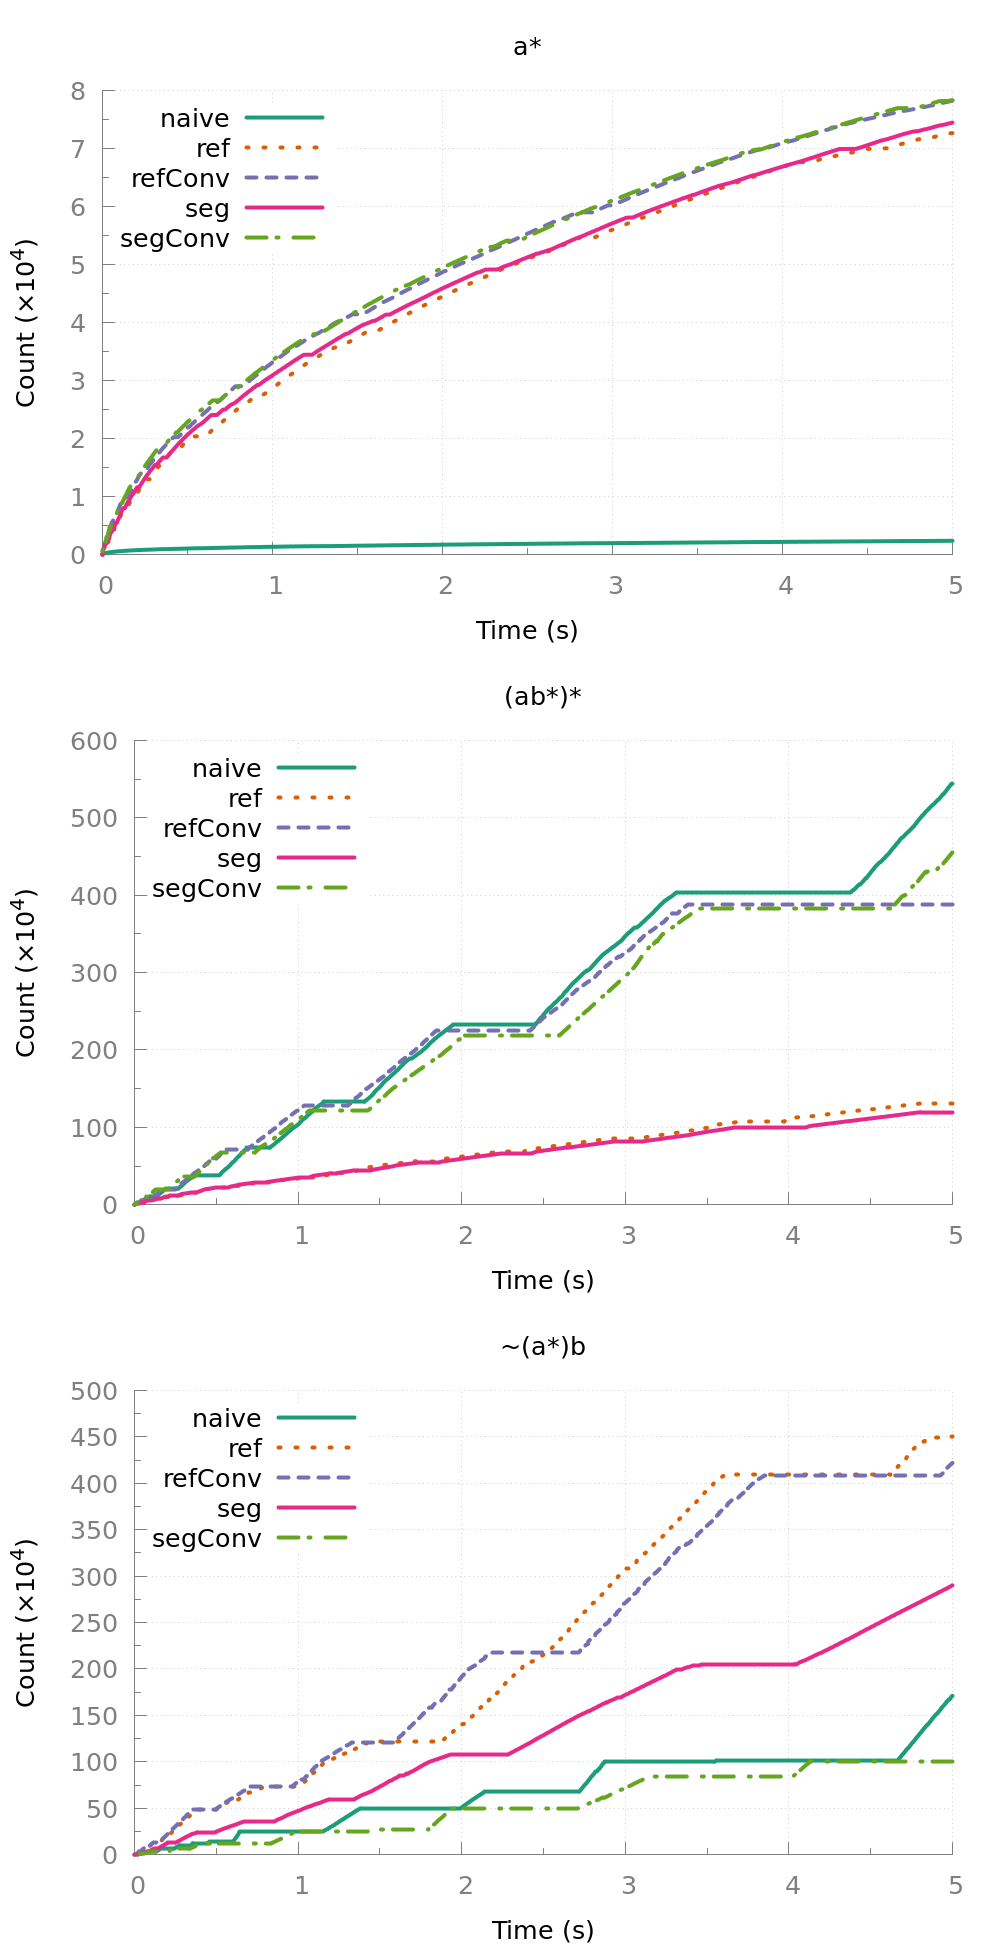
\includegraphics[width=\linewidth]{measure/haskell_all.png}
  \caption{Benchmark for the \haskell implementation with various algorithms}
  \label{bench:haskell:all}
\end{figure}

We consider five variants of the Haskell implementation.
\begin{itemize}
\item \textbf{McIlroy} our implementation of \citet{DBLP:journals/jfp/McIlroy04}. 
\item The \textbf{seg} implementation uses the infinite list-based segmented
  representation throughout (\cref{sec:segm-repr}).
\item The \textbf{segConv} implementation additionally
  applies the convolution approach (\cref{sec:convolution,sec:faster-closure}).
% \item The \textbf{ref} implementation uses symbolic segments
%   from \cref{sec:more-finite-repr} combined with
%   maps and sparse indexing.
\item The \textbf{refConv} implementation combines
   symbolic segments (\cref{sec:segm-repr,sec:more-finite-repr}) with the convolution approach.
\end{itemize}

Performance is evaluated by iterating through the stream of words
produced by the generator, forcing their evaluation\footnote{In
  Haskell, forcing is done using \lstinline{Control.DeepSeq}.}
and recording the elapsed timed every 20 words for 5 seconds.
The resulting graph plots the time (x-axis) against the number of words (y-axis) produced so far. The slope of the graph indicates the generation speed of the algorithm, high slope is correlated to high generation speed.  \cref{bench:haskell:all} contains the results for the Haskell implementations.
 
Most algorithms generate between $1.3\cdot10^3$ and $1.4\cdot10^6$ words in the first
second, which seems sufficient for testing purposes.
The \textbf{refConv} implementation
which uses symbolic segments and convolutions is consistently in the
leading group.
% Sometimes one of the other implementations is slightly
% faster, but not consistently so.
This observation validates that the
changes proposed in \cref{sec:improvements} actually lead to
improvements.
%
Looking at each graph in detail, we can make the following
remarks:
\begin{itemize}[leftmargin=*]
\item All implementations are equally fast on $\Rstar a$ except
  \textbf{McIlroy}, which implements star inefficiently.
\item The graph of some implementations
  has the shape of ``skewed stairs''. We believe this phenomenon is due to
  insufficient laziness: when arriving at a new segment, part of the
  work is done eagerly which causes a plateau. When that part is done,
  the enumeration proceeds lazily.  As laziness and GHC
  optimizations are hard to control, we did not attempt to correct this.
\item The expression $\Rstar{(\Rconcat{a}{\Rstar{b}})}$ demonstrates that
  the convolution technique presented in \cref{sec:convolution}
  leads to significant improvements when applying \code{star} to non-sparse languages.
\item The \textbf{refConv} algorithm is
  significantly faster on $\Rconcat{\Rcomplement{(\Rstar{a})}}{b}$
  compared to \textbf{seg} and \textbf{segConv}. We have no good
  explanation for this behavior as the code is identical up to the
  symbolic representation of full and empty segments. However, the
  only sublanguage where this representation could make a difference
  is $\Lang{b}$, which is also represented finitely by
  \textbf{segConv} and should thus benefit from the convolution
  improvement in the same way as \textbf{refConv}.
\item The expression $\Rintersect{\Rcomplement{(\Rstar{a})}}{\Rcomplement{(\Rstar{b})}}$
  shows that all our algorithm have similar performance profiles on
  set-operation. They are also significantly faster than
  \textbf{McIlroy}.
\end{itemize}


\subsection{Comparing Data Structures in the \ocaml Implementation}
\label{sec:bench:ocaml}
\begin{figure}[!tb]
  \centering
  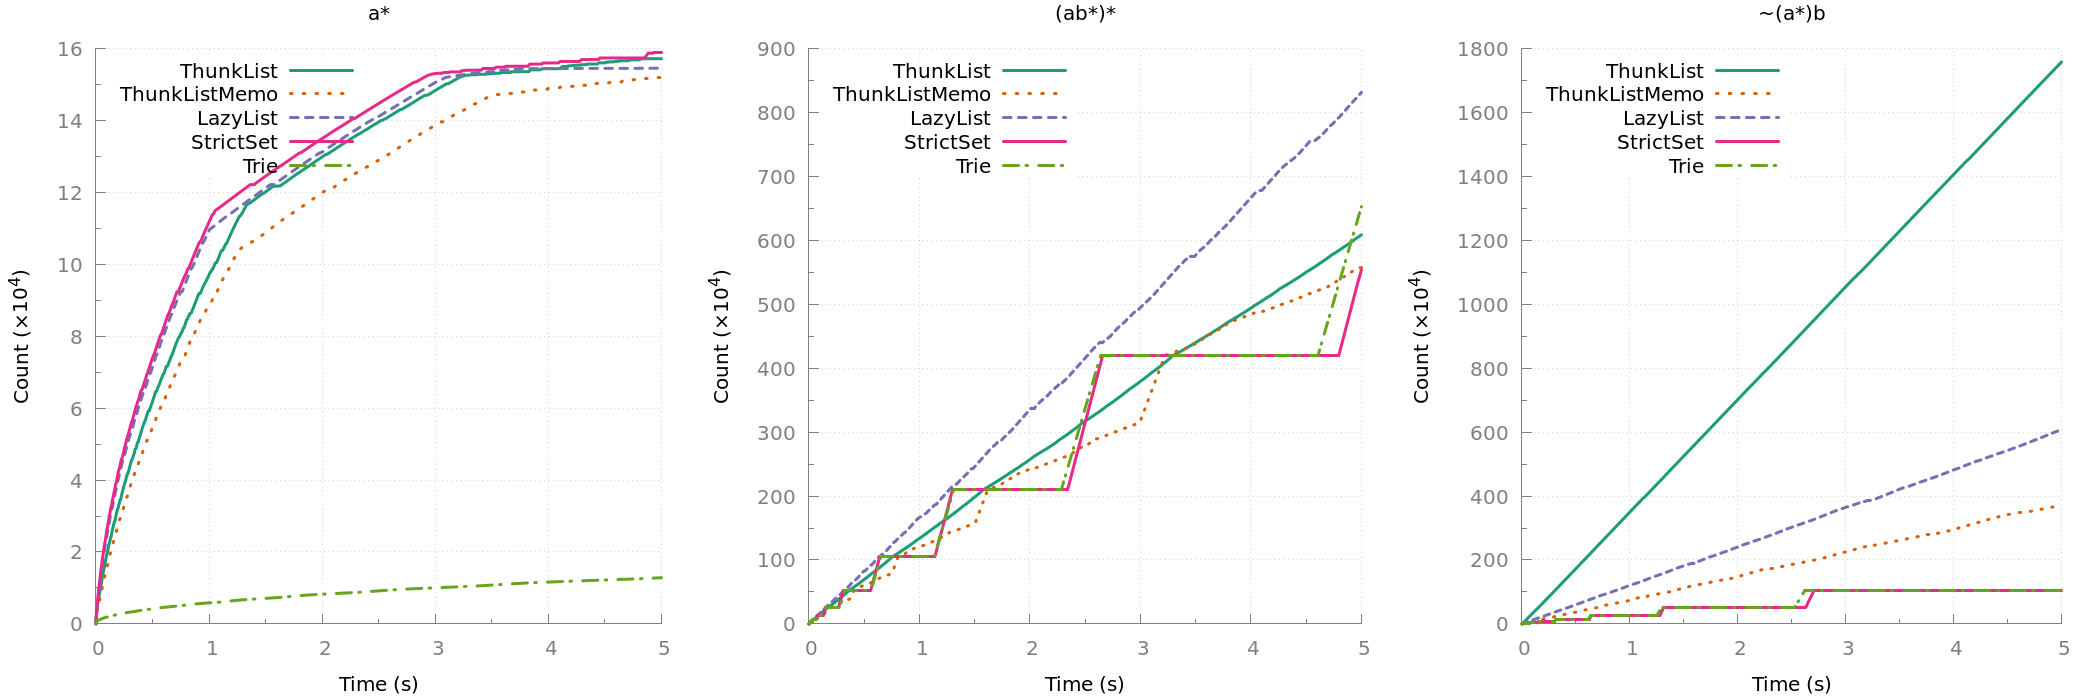
\includegraphics[width=\linewidth]{measure/ocaml_all.png}
  \caption{Benchmark for the \ocaml implementation with various data-structures}
  \label{bench:ocaml:all}
  \label{bench:ocaml:union}
\end{figure}

We have now established that the \textbf{refConv} algorithm
provides the best overall performance.  The \haskell implementation,
however, uses lazy lists to represent segments.
To measure the influence of strictness and data structures on
performances, we conduct experiments with the functorized \ocaml implementation.
We follow the same methodology as the \haskell evaluation using the
regular expressions $\Rstar a$, $\Rstar{(\Rconcat{a}{\Rstar{b}})}$ and
$\Rconcat{\Rcomplement{(\Rstar{a})}}{b}$.  The results are shown in
\cref{bench:ocaml:all}.

Unlike the previous benchmark for algorithms, there is no clear winner
among the data structures.
Lazy and Thunk lists, with or without memoizations, are the most ``well-rounded''
implementations and perform decently on most languages.
% We can however make the following remarks.
\begin{itemize}[leftmargin=*]
\item The \code{Trie} module
  is very fast thanks to its efficient concatenation.
  It performs badly on $\Rstar a$
  due to the lack of path compression:
  in the case of $\Rstar a$, where each segment contains only one word, the
  trie degenerates to a list of characters.
  We believe an implementation of tries with path compression would perform
  significantly better.
\item The other data structures exhibit a very pronounced slowdown on $\Rstar a$
  when reaching 150000 words.
  We believe this slowdown is due to garbage collection because
  the active heap contained 10G of data before
  a collection was triggered. Far less memory is consumed for other languages.
\item Strict data structures showcase a marked ``skewed
  stair'' pattern, which is completely absent for \code{ThunkList} and
  \code{LazyList}. Thus, manual control of laziness works well in
  \ocaml. These results also demonstrate that strict data structures
  should only be used when all elements up to a given length are
  needed. In such a case the stair pattern causes no problems.
\item Memoization for thunk lists does not significantly improve performance.
  It seems that the linear cost of memoizing the thunk list and
  allocating the vectors
  is often higher than simply recomputing the lists.
\item The expression $\Rstar{(\Rconcat{a}{\Rstar{b}})}$ shows that sorted enumerations and tries
  perform well on set-operations, even compared to strict sets.
\end{itemize}

\subsection{The Influence of Regular Expressions on Performance}
\begin{figure*}[!tp]
  \centering
  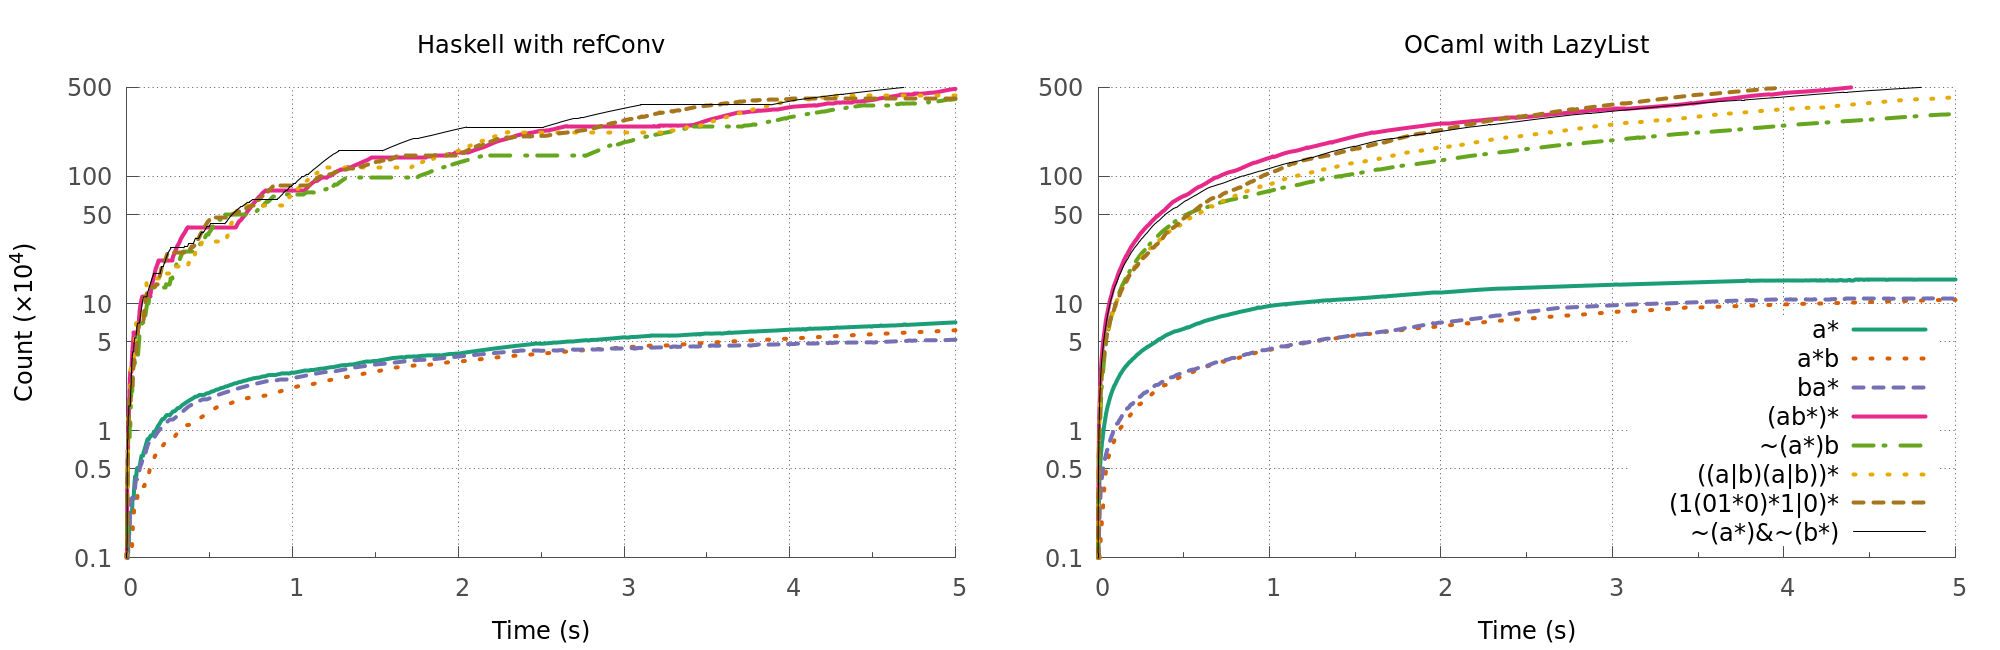
\includegraphics[width=\linewidth]{measure/langs.png}
  \caption{Benchmark on different regular expressions}
  \label{bench:langs}
\end{figure*}

The benchmark results so far demonstrate that the performance of the language
generator highly depends on the structure of both
the generated language and the regular expression considered.
To further explore this observation we compare a range of regular expressions
with the \code{refConv} \haskell implementation and the \code{LazyList}
\ocaml implementation.
Before presenting the results, a word of warning:
We do not claim to offer a fair comparison between languages!
The two implementations are not exactly the same and we made no attempt
to measure both languages under exactly the same conditions.
%
\cref{bench:langs} contains the results with a
logarithmic scale for the word count as it enables better comparison
between the regular expression specimens.

We add three new regular expressions to the range of expressions already considered:
\begin{itemize}
\item $\Rstar{(\Sigma\Sigma)}$, the language of words of even
  length. This language is neither finite nor cofinite, but it can make
  good use of the symbolic representation of segments.
  % \footnote{This
  %   language has $P (w \in L) = 0.5$ thus solving the exercise posed
  %   earlier.}
\item $\Rstar{(\Runion{1 \Rstar{(0\Rstar{1}0)}1}{0})}$, the language
  of multiples of 3 in binary representation. Again, this is a language that is neither
  finite nor cofinite, but its segments are never full nor empty.
\item $\Rstar{a}b$ and $b\Rstar{a}$, which together check whether
  the performance of {concatenation} is symmetric.
\end{itemize}

Languages are roughly ordered by size/density, i.e., $P (w\in L)$. We
observed that the bigger the segments of a language, the faster it is
to generate its words.  If each segment contains many words, we do not
need to compute many segments to generate a large number of words.
Moreover, most operations, notably those involving the product of
segments, are more expensive when considering segments of higher
indices. Briefly put, long strings are harder to generate than short
ones.
%
Regarding symmetry, we find that the generation of $\Rstar{a}b$ and
$b\Rstar{a}$ has the same performance in both implementations,
thanks to the improved convolution technique
with detection of finite languages described in \cref{sec:convolution}.



%%% Local Variables:
%%% mode: latex
%%% TeX-master: "main"
%%% End:
